\chapter{Flexibility-based AC-Optimal Power Flow for active network management in distribution grids}
\label{ChapterOPFDSO}
\chaptermark{Optimal Power Flow for Distribution System Operators}

\section{Introduction}

The dynamics of the power system are changing towards a new model where large generators on the high-voltage side of the network are being replaced by smaller generation units placed at the medium-voltage and low-voltage side of the grid. This increase of penetration by DERs will have a significant impact on how the distribution network operates. At the distribution level, distributed energy resources will make arise some new challenges and, in some cases, problems already solved will rise again. As a result, the increasing number of DERs placed alongside the medium-voltage  and low-voltage distribution networks leads to the need of flexibility services for the DSO. 
This chapter aims to develop an optimization tool for calculating the value and location of the flexibility request that a DSO needs for operating the distribution network and avoid or mitigate network congestions, corresponding to objective $(iv)$ of the thesis research, according to Figure \ref{fig:chapter_obj_iv}. 

\begin{figure}[htbp]
	\centering
	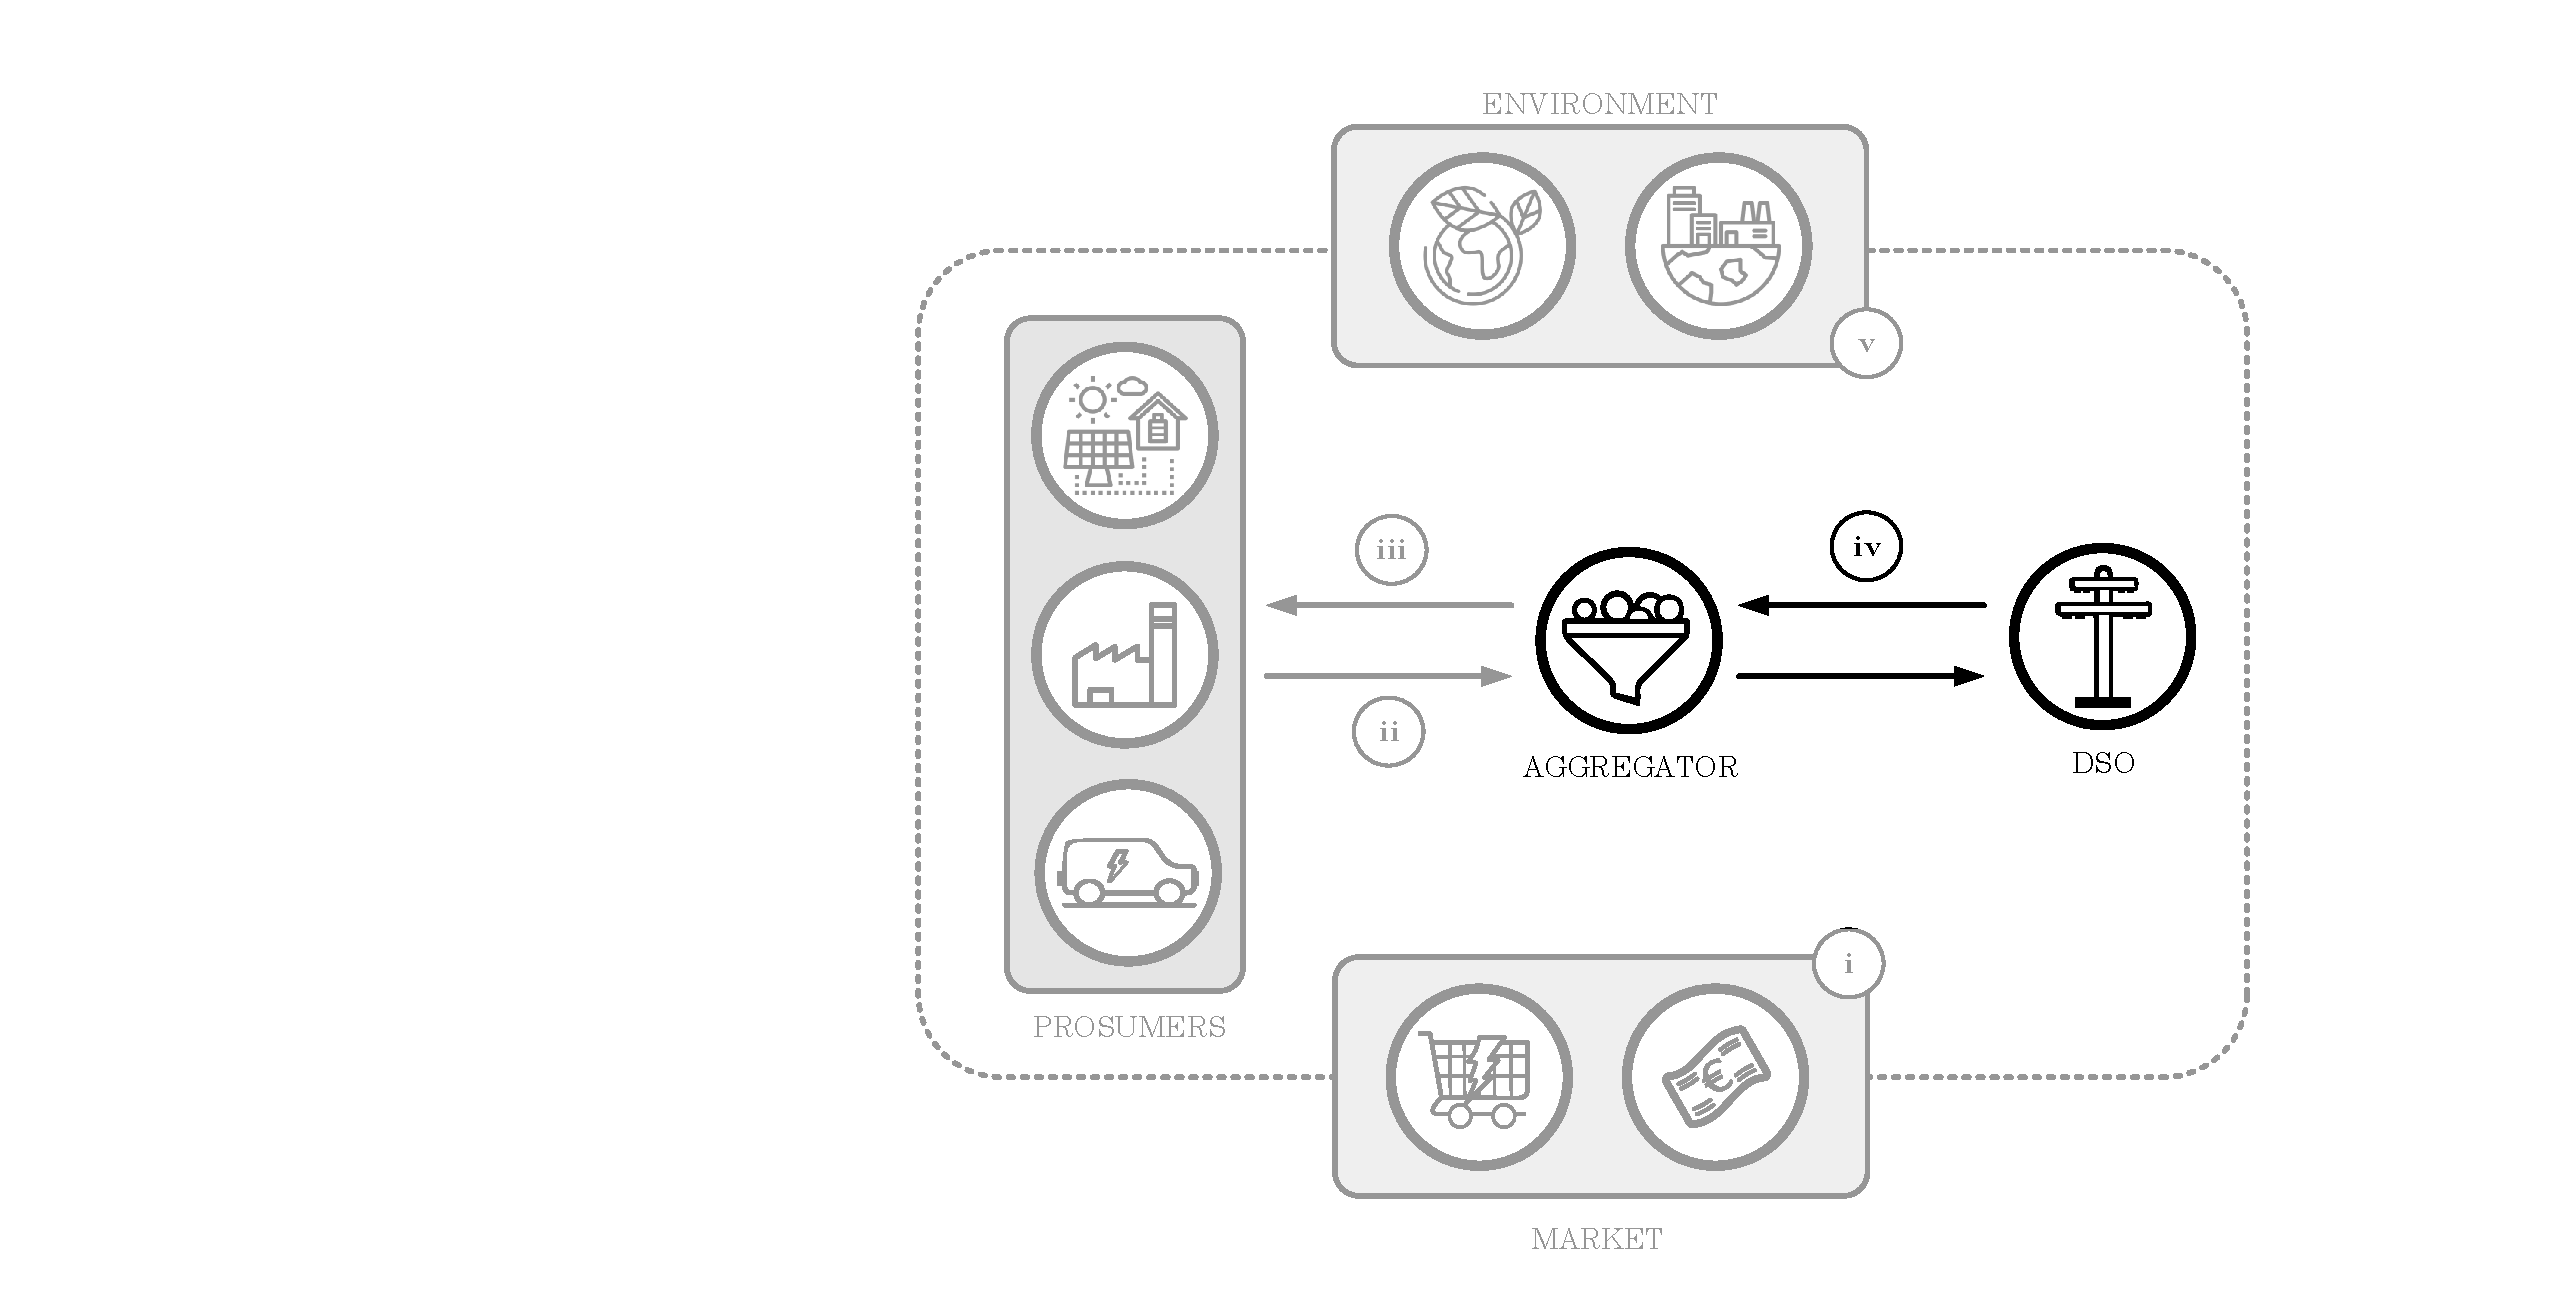
\includegraphics[width=0.7\columnwidth ]{ChapterOPF_DSO/Figures/phd_intro_iv.pdf}
	   %\vspace*{-8cm}
		\caption{Chapter objective based on the PhD scope}
	\label{fig:chapter_obj_iv}  
\end{figure}

These flexibility services could be provided by several resources, from different nature, including centralized energy storage, distributed energy storage, electric vehicles, PV panels, or Flexible Loads such as water boilers or space heaters [3]. The aggregator gathers the flexibility from customers to provide flexibility services to different stakeholders, like energy suppliers, Balance Responsible Parties (BRP), TSO, DSO and final consumers (\cite{USEFFoundation2015a, Olivella2018}). Then, the aggregator acts as a single entity when engaging in power system markets or selling services to the system operators \cite{BURGER2017}. Under the context of smart grids and flexibility services in place, distribution system operators could benefit by activating flexibility in distribution grids \cite{USEFFoundation2015a, spiliotis2016demand, esmat2016conf, hashemi2016}. DSOs could compensate grid congestions during high consumption or production periods, reducing their networks stress. At the same time, DSO can increase their renewable generation hosting capacity by using behind-the-meter flexibility during peak production periods. 

The most common problems caused by the high penetration of distributed and renewable generation can be classified into four main categories. Figure \ref{fig:network_problems} provides an overview of the location of these potential problems in a arbitrary distribution network, also detailed in the following list:  

\begin{enumerate}
\item Overload and losses of feeders and transformers. 
\item Risk of overvoltage.
\item Power quality disturbances.
\item Incorrect operation of protection elements. 
\end{enumerate}

\begin{figure}[h]
	\centering
	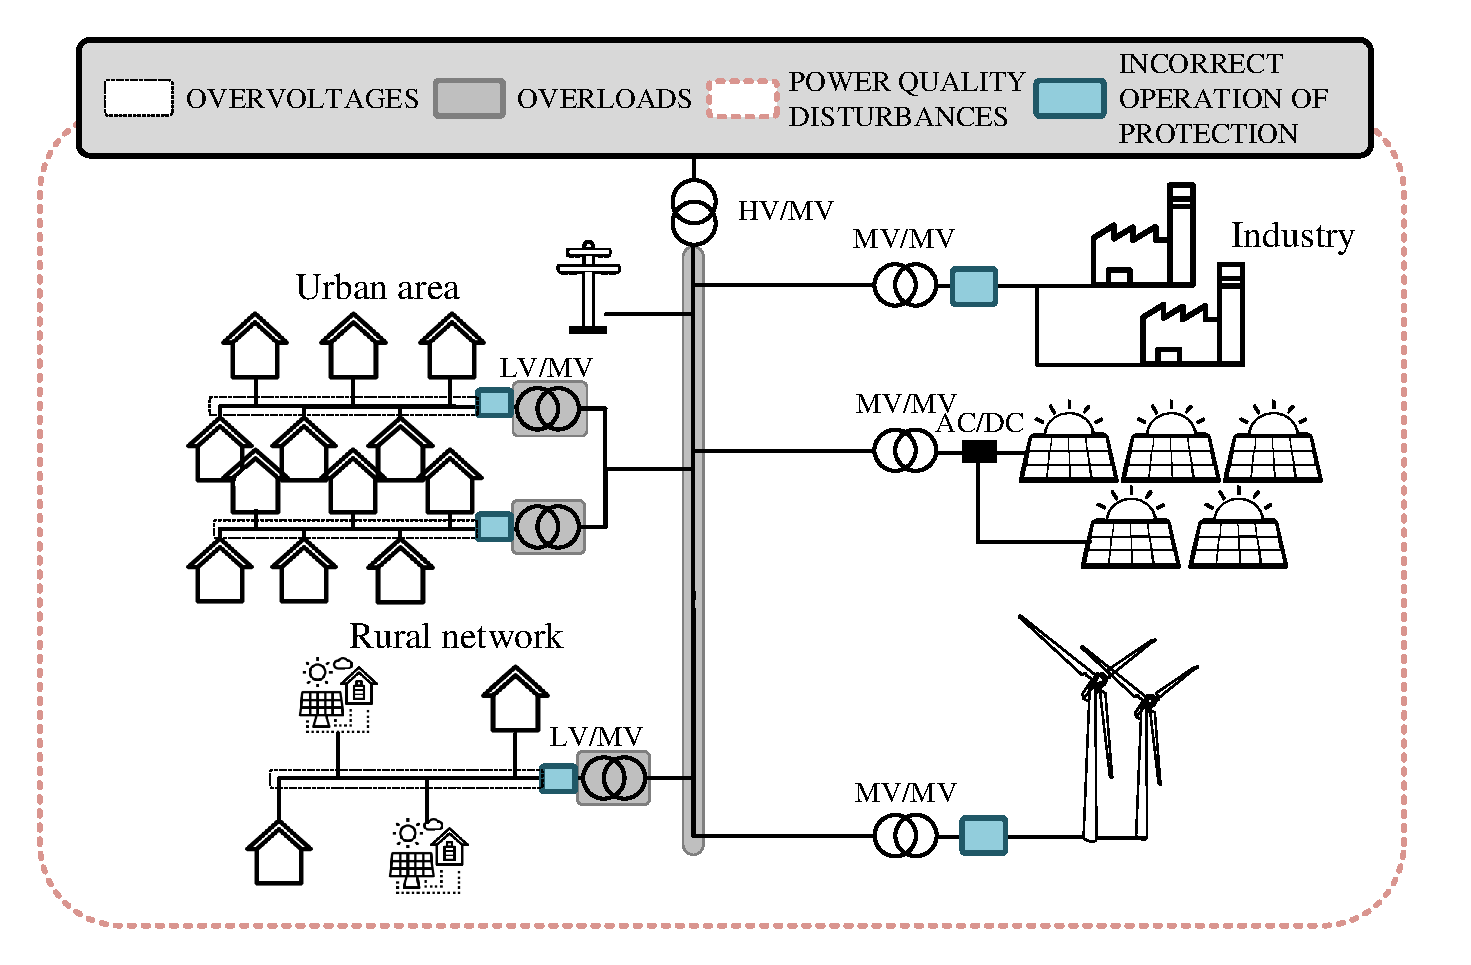
\includegraphics[width=1\columnwidth]{ChapterOPF_DSO/Figures/network_problems.pdf}
	   %\vspace*{-8cm}
		\caption{Distribution network scheme with potential problems and areas}
	\label{fig:network_problems}  
\end{figure}

Based on previous references \cite{ISMAEL20191002, Bollen2011}, the two main potential problems under the distribution network operation are $(i)$ \textbf{overload} and  $(ii)$ \textbf{overvoltage}. The following sections defines the potential problems and details the main causes of them. 


\subsection{Risk of overload/overcurrents - congestion management}
Overloads or commonly also known as overcurrents are those situations where the current circulating through one of the electrical components is higher than the nominal value. This can cause either the damage of the electrical component if the situation happens for a short period of time, or the component failure if the current limit is overly exceeded. However, in many cases, protection elements would trigger and interrupt the service so as to guarantee the correct performance of the component. 
If we consider the current scenario of energy transition with a high penetration of DERs, the risk of overcurrent is mainly caused by the increase of the electricity consumption in a network that has not been reinforced since its construction, and the increase of DERs and electrical appliances such as space heaters, electric vehicles and electric water boilers. In the latter case, the electricity in injected usually at MV and LV levels. In this scenario, overloads can happen when the overall resulting power flow downstream the distributed generator point exceeds the value upstream, under the hyphoteses that no other generation sources are providing energy. This is also related to the feeder capacity limits under normal operation schemes. The scenario where a feeder capacity has been working at its 40-50\% capacity before the integration of capacity generation would have a wider range to allocate these resources than those feeders that in normal operation are at its 90-95 \% of the total capacity. Furthermore, the length of the feeder should be also taken into consideration, since at the beginning of the power line the electricity to be distributed must be equal to the sum of all loads, whereas at the end of the feeder only the remaining has to be provided. Hence, the feeder capacity is also related to the length, structure and connected loads. 
Despite the disadvantages and challenges of DERs in distribution networks, it is a fact that DERs can help reduce the losses in the electricity system, since generation is now closer to the consumption points. However, it should be considered that under the case of an excess of generation, reverse flows in MV and LV lines can increase the power losses of the overall system. 

\subsection{Risk of overvoltage - voltage control}
The second most common risk in active distribution grids are overvoltages. This situation takes place when the voltage value at one or more of the buses exceeds the nominal value. As in the case of overloads, if the overvoltage is too high, this can lead to the damage of the electrical components and the electric loads connected to that bus. 
For many years, voltage magnitude variations have been a common concern for system operators being the case of undervoltages. This problem is caused by the associated impedance in the distribution lines leading to an excessive voltage droop, but it does not cause any damage to the network components.  

With the increase of DERs integration, utilities have registered an increase of overvoltage cases at the point of common copuling (PCC) of DERs units, and as a result have set up limits on the maximum size of a distributed generator \cite{Kennedy2014}. The reason being is that these grid-connected distributed generators unit do not explicitly regulate voltage, most commonly regulating the real power output. One of the mitigation schemes for overvoltages is the previously mentioned one, stablishing restrictions on the distributed generator size and location, under the expansion and planning process of the network. However, with the aim of enhancing the integration of DERs, this could lead to a lack of fairness for end-users who are willing to install DERs at a household or LV-MV level. Another mitigation scheme is the combination of DERs with storage units, avoiding the risk of overvoltage by using the battery to manage the energy surplus. Lastly, demand-side management techniques and flexibility can help the mitigation of overvoltages in active distribution networks. 

\section{Demand-side flexibility for congestion management}
As mentioned in the previous section, the use of demand-side flexibility, managed by aggregators, can help distribution network operators avoid or mitigate congestions. 

%RESEARCH QUESTION: INCLOURE FEINA DEL PAPER DEL CIRED

\textcolor{red}{The idea here is to use the demand forecast as well as the network congestion input to compute and calculate the flexibility request that the DSO requires for solving the congestion located in a specific point of the network}
\textcolor{red}{This service does not interact with the aggregator and we do not consider the interaction between the agents (S5.3) BD4OPEM}

%\begin{itemize}
%\item NUVVE Congestion management
%\item pilot estabanell INVADE - BD4OPEM 
%\item altres pilots
%\end{itemize}

\subsection{System interaction}
The DSO is responsible for calculating their Flexibility Requests (FR) for congestion management purposes. On the other hand, the FO is the responsible for calculating the flexibility offers, which can cover partially or entirely the DSO needs. Hence, an interaction between the DSO and the FO is needed to activate the required flexibility services. The data flow is depicted in Figure 2 below.

\begin{figure}[h]
	\centering
	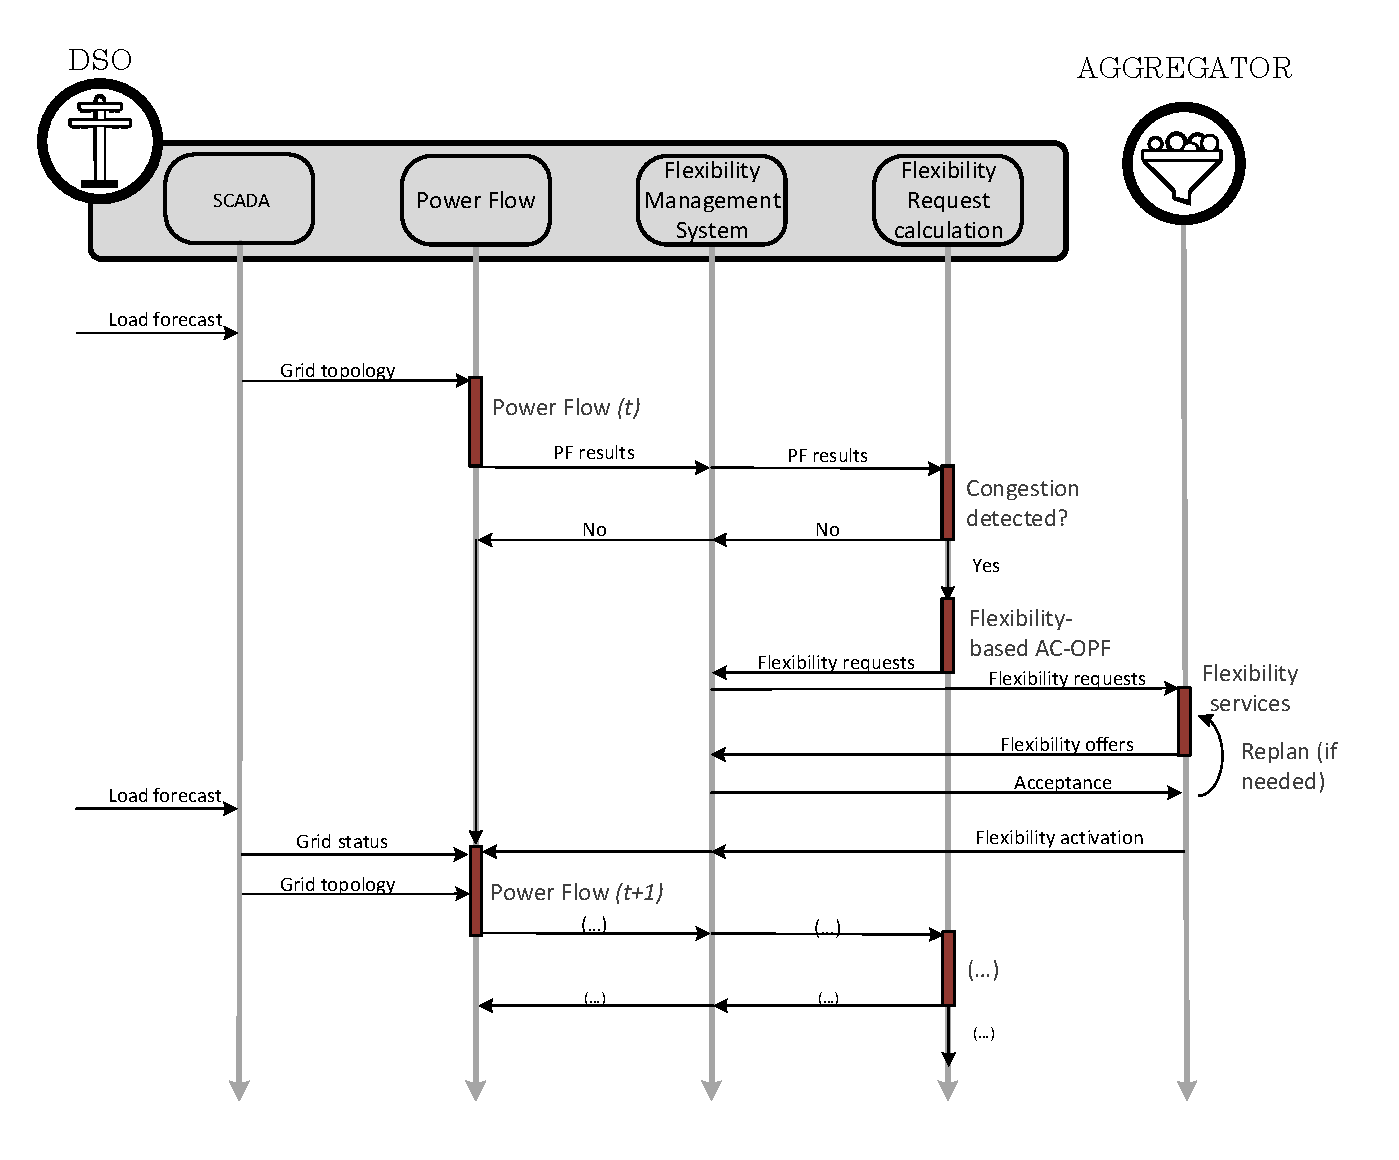
\includegraphics[width=1\columnwidth ]{ChapterOPF_DSO/Figures/OPF_interaction_ACOPF.pdf}
	   %\vspace*{-8cm}
		\caption{Flexibility request interaction}
	\label{fig:pimodel}  
\end{figure}

%\subsection{Standards and protocols for flexibility provision between aggregators and DSOs}
%OPENADR - USEF? 
%\subsection{Literature review on congestion management tools - OPF}
%\subsection{Contribution}
\section{Contribution}

The optimization problem is developed to minimize the aggregator operation costs. The costs are based on curtailing local generation output, charging or discharging batteries, switching off curtailable and disconnectable loads and shifting loads during specific time periods. A local flexibility market design is presented in [12], described as a market-based mechanism for aggregators. BRP and DSO are the main stakeholders of these flexibility services and they can buy flexibility from a market platform or a bilateral contract. However, in any case an information exchange is required between the flexibility buyer and the flexibility provider, to agree on the quantity and delivery time of this flexibility to be provided. 

\section{Flexibility activation costs for distribution network operators}
\textcolor{red}{incloure coses nuria aqui. caldra lincarho amb la part de parametres, del parametre de costos de la funcio objectiu.} 

\section{Mathematical formulation for Flexibility request calculation}
The problem to solve is mainly an AC-OPF, considering as the objective function the minimization of the total flexibility activation costs, but also considering the distribution network related constraints. The following section outlines the formulation, convering the objective function and the related constraints of the model.
This AC-OPF formulation is based  on the polar Power-Voltage formulation XXXX. This formulation represents complex quantities in polar form, and explicitly uses sines and cosines in the power flow constraints. However, in this case the objective function as well as some of the nodal power balance and the power at buses is adapted to the objective of the flexibility provision for DSOs.

This chapter will consider the notation for complex magnitudes such as voltage at each of the buses, $\underline{V}_{i,t}$. The polar formulation of this variable can be hence outlined as follows

\begin{equation}
\underline{V}_{i,t} = V_{i,t} \phase{\theta_{i,t}}
\end{equation}

where $V_{i,t}$ represents the module and $\theta_{i,t}$ the angle in rad. In the case of the Bus Admittance, $\underline{Y}_{ik}$, the physical representation of the line admittance can be formulated as

\begin{equation}
\underline{Y}_{ik} = G_{ik} + jB_{ik}
\end{equation}

where $G_{ik}$ is the conductance of the line and $B_{ik}$ is the susceptance, both measured in siemens $[\omega^{-1}]$. $\underline{Y}_{ik}$ can also be formulated as a Line Admittance Matrix, $[Y]_{bus}$, an $N x N$ matrix, where $N$ is the number of nodes. This matrix composed by all the nodal admittance of the various buses. It explains the topology and the admittance of the network. It is a symmetric matrix and the way to obtain the elements of this matrix follow the criteria listed below:

\begin{subequations}
\begin{align*}
& \underline{Y}_{bus_ii}= y_sh,i + \sum_k y_{ik} \\
& \underline{Y}_{bus_ij} = - \sum y_{ij}
\end{align*}
\end{subequations}

Where $i$ and $j$ are buses of the network, and $k$ are all the buses connected to bus $i$. For the sake of simplicity, we will consider $[Y]_{bus}$ as $[Y]$, being each of the elements in the matrix the i-j element a complex number $\underline{Y}_{bus_ij}$. In the case of distribution networks, being it the case of study in this chapter, the equivalent network scheme in order to obtain the line admittances is based on the $\pi$-model, shown in Figure \ref{fig:pimodel}. This equivalent scheme considers both the series impedance, $z_{ik}$, and the shunt admittance $y_{ik_1}$ and $y_{ik_2}$ 

\begin{figure}[]
	\centering
	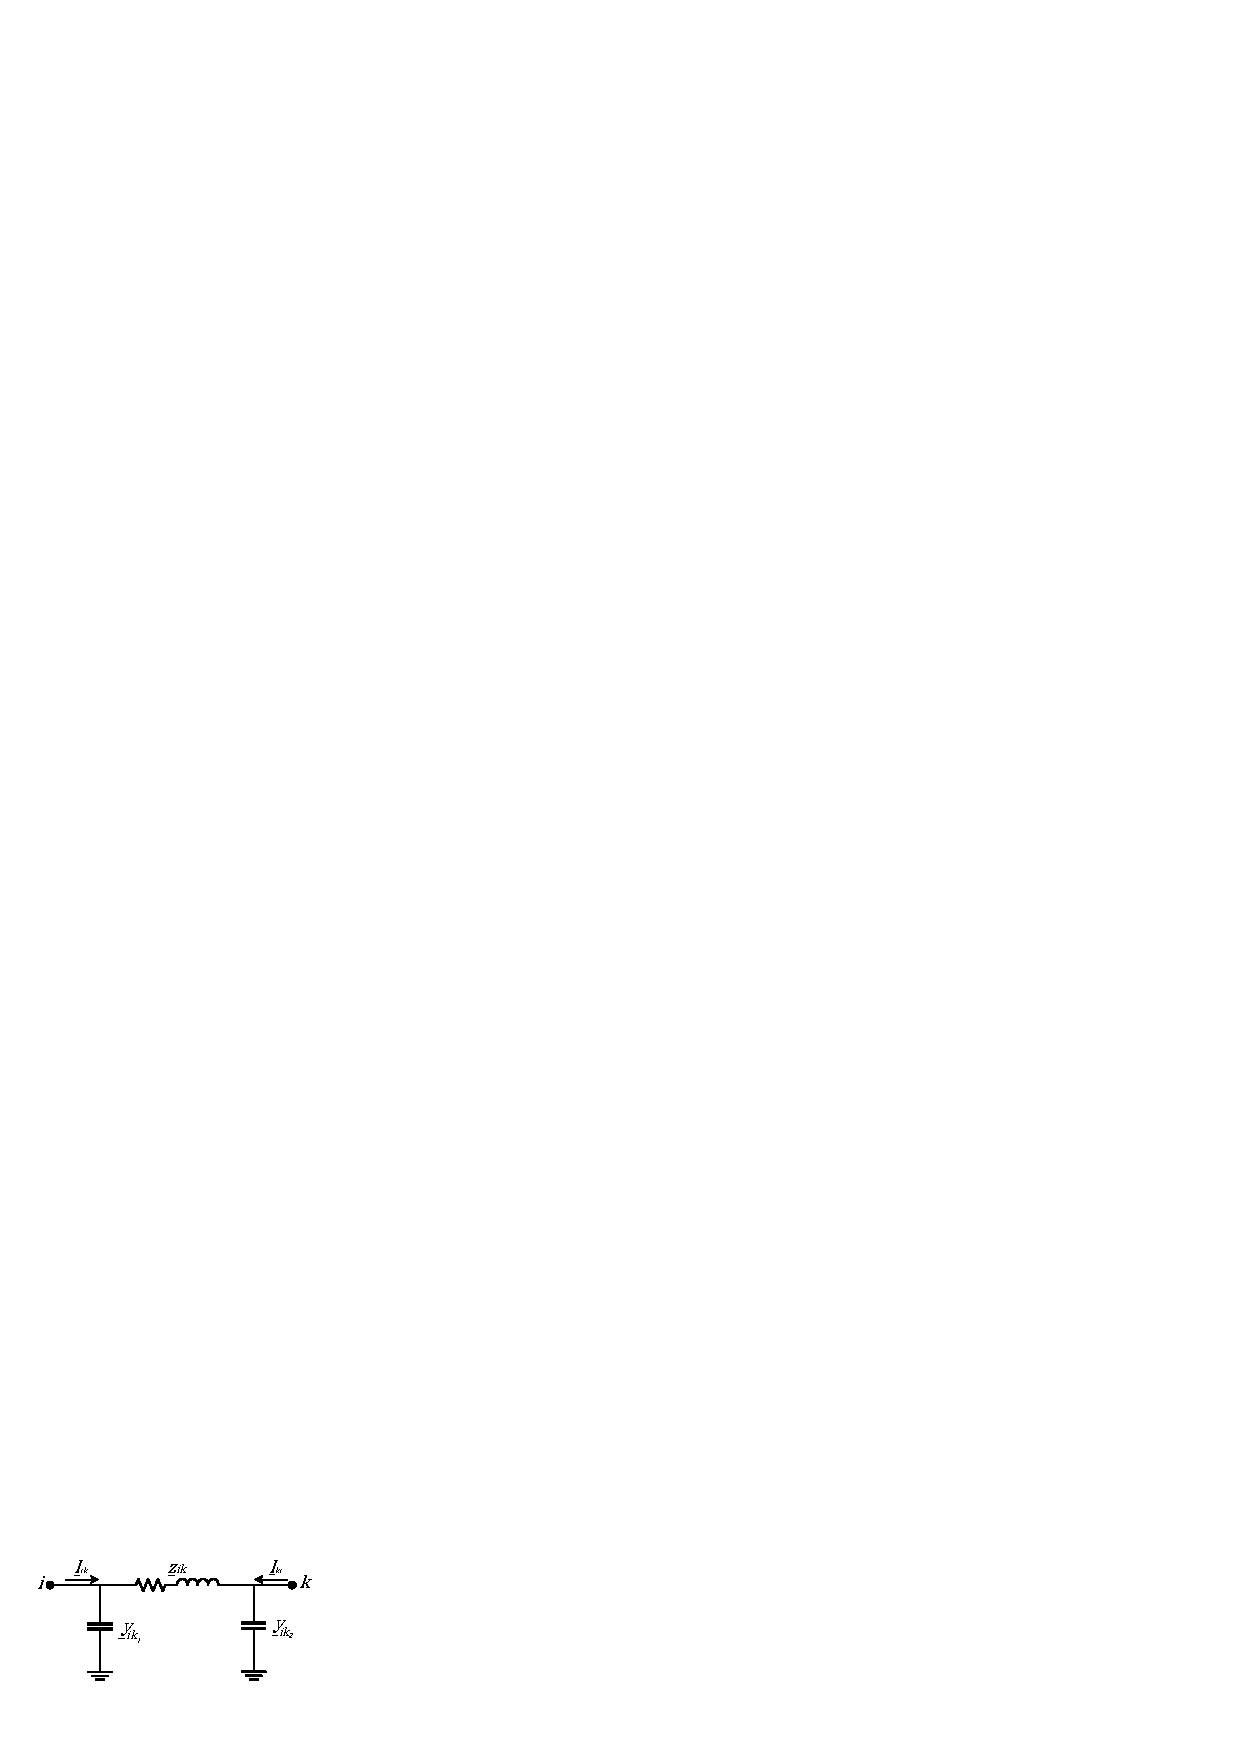
\includegraphics[width=0.7\columnwidth ]{ChapterOPF_DSO/Figures/pimodel2.pdf}
	   %\vspace*{-8cm}
		\caption{$\pi$-model of the network}
	\label{fig:pimodel}  
\end{figure}

In all cases, the relationship between the nodal admittance matrix  $[Y]_{bus}$ and the nodal impedance matrix  $[Z]_{bus}$ is maintained following the following equation 

\begin{equation}
[Y]_{bus} = [Z]_{bus}^{-1}
\end{equation}


The apparent power of the line, $\underline{S}_{i,t}$, measured in VA, can be decomposed into active,$P_{i,t}$ in W, and reactive power $Q_{i,t}$ in var, by the following equation 

\begin{equation}
\underline{S}_{i,t} = P_{i,t} + jQ_{i,t}
\end{equation}


%\subsection{Objective Function}
The objective function is to minimize the total flexibility costs function. This function is based on the price accorded between the FO and the DSO for period $t \in T$, $C_{t}^{flexDSO}$ and the total active power injected by the flexibility resource, $\phi_{i,t}^{ACT}$ .

\begin{equation*}
\!\min_{P_{i,t}, Q_{i,t}, \theta_{i,t}}  \qquad \sum_{t}^{T} \left( \sum_{i}^{N} C_t^{flexDSO} \cdot \phi_{i,t}^{ACT} \right)  
\end{equation*}

%\subsection{Constraints}
The constrains listed below ensure the compliance of the AC Power Flow equations and a correct system operation.
The AC power flow equations describe the power system network operating point in steady state and are based on complex phasor representation of voltage-current relationship at each node. The active $P_{i,t}$ and reactive $Q_{i,t}$ power flow node balance at node $i \in K$ in period  $t \in T$, are formulated below Eq. XXXX and Eq. XXX. Then, Eq. XXX details the mathematical conversion to express  $\theta_{i,k,t}$ from the voltage angle at each node.

\begin{subequations}
\begin{align*}
& P_{i,t} = V_{i,t} \sum_{k=1}^{N} V_{k} (G_{i,k} \cos(\theta_{i,k}) + (B_{i,k} \sin(\theta_{i,k})) \qquad \forall i,\forall t  \\ 
& Q_{i,t} = V_{i,t} \sum_{k=1}^{N} V_{k} (G_{i,k} \sin(\theta_{i,k}) - (B_{i,k} \cos(\theta_{i,k})) \qquad \forall i,\forall t \\
& \theta_{ik,t} = \theta_{i,t} - \theta_{k,t} \quad   \qquad  \forall t \\
& P_{i,t} = P_{i,t}^{G} - P_{i,t}^{D}  \quad   \qquad  \forall t  \\
& Q_{i,t} = Q_{i,t}^{G} - Q_{i,t}^{D}  \quad   \qquad  \forall t  
\end{align*}
\end{subequations}


Since the pilot-site is considering sources connected at each node of the grid, the total active power at node $i \in K$ in period $t \in T$, $P_{i,t}$, considers the active power generated, the active power demanded and the active power injected by the flexibility source Eq. XXXXX. Regarding the reactive power, Eq. XXXX also considers the reactive power generated at node  $i \in K$ in period $t \in T$ the reactive power consumed at node $i \in K$ in period $t \in T$ and the reactive power consumed or injected by the flexibility source.
Hence, from the admittance equations, it is possible to calculate the apparent flow injected depending on the voltages at all the grid nodes Eq. XXXXX. Consider that the underscore means that the parameter or variable is a complex number. Whether the variable or the parameter is not written with an underscore, a real value is considered.

The line flow constraints follow the $\pi$-model of the grid, since both the longitudinal impedance and the transversal capacitance of the line have to be considered in the case of MV networks and AC-OPF. For the sake of clarity, the $\pi$-model is shown in \ref{fig:pimodel}. Each line of the distribution network is limited to the maximum allowed line current, $I_{l}^{MAX}$


\begin{subequations}
\begin{align*}
& \underline{S}_{ik} = \underline{V}_{i} \cdot \underline{I}_{ik}^{*} = \underline{V}_{i} \left[ \frac{\underline{V}_{i} - \underline{V}_{k}}{\underline{z}_{ik}} + \underline{V}_{i} \; \underline{y}_{ik_1} \right]^{*}   \qquad  \forall t  \\
& \underline{S}_{ki} = \underline{V}_{k} \cdot \underline{I}_{ki}^{*} = \underline{V}_{k} \left[ \frac{\underline{V}_{k} - \underline{V}_{i}}{\underline{z}_{ik}} + \underline{V}_{k} \;  \underline{y}_{ik_2} \right]^{*}   \qquad  \forall t  
\end{align*}
\end{subequations}

The parameters $\underline{y}_{ik_1}$,  $\underline{z}_{ik}$ and $B_{i,k}$

The flexibility sources have both the possibility to inject or consume active power, according to up-regulation or down-regulation commands, to mitigate congestions along the distribution grid. Hence, each source is connected to a node $i \in K$, and each node will have an upper and lower active power limitation, $-P_{i,t}^{flex,MIN}$ and $P_{i,t}^{flex,MAX}$  in time period $t \in T$.

Reactive Power bounds by the flexibility source
The flexibility sources connected at node $i \in K$, are able to inject or provide reactive power, $\phi_{i,t}^{REA}$. Hence, this variable is restricted between $-Q_{i,t}^{flex,MIN}$ and $-Q_{i,t}^{flex,MAX}$.

\begin{subequations}
\begin{align*}
&  0 \leq P_{i,t}^{G} \leq P_{i,t}^{G,MAX}  \quad   \qquad  \forall t  \\
&  - Q_{i,t}^{G,MAX} \leq Q_{i,t}^{G} \leq Q_{i,t}^{G,MAX}  \quad   \qquad  \forall t \\
\end{align*}
\end{subequations}

\textcolor{red}{Review this paragraph}
The apparent power limitation S is not considered in this mathematical formulation. The active and reactive power limitations are considered as technology free. That means that the total amount of reactive and reactive power in each node is limited, but not considering each technology itself. Hence, some sources can provide $\phi_{i,t}^{ACT}$ like PV and  batteries and, other sources provide $\phi_{i,t}^{REA}$ like DR and EV. The DSO does not consider the technology itself and its capacity limitations. The FO is the entity  responsible for that. 

\begin{subequations}
\begin{align*}
&  S_{ik,t} \leq S_{ik,t}^{MAX}  \quad   \qquad  \forall t  \\
&  S_{ki,t} \leq S_{ki,t}^{MAX}  \quad   \qquad  \forall t  \\ 
\end{align*}
\end{subequations}

In the AC-OPF algorithm, the nodal voltage is restricted by an upper limit and a lower bound to guarantee the correct operation of the system. In the flexibility requests calculation algorithm, the DSO contracts the flexibility services to prevent and mitigate congestions along the distribution grid. Hence, the DSO aims to minimize the congestion risks throughout the day, which can vary. For this reason, the voltage upper and lower bounds parameters consider also the time period $t \in T$, resulting in the following parameters, $V_{i,t}^{MIN}$ and $V_{i,t}^{MAX}$. These parameters will be provided by the DSO based on the level of risk they want to assume on congestions along the network.

\begin{equation*}
V_{i,t}^{MIN} \leq V_{i,t} \leq V_{i,t}^{MAX}  \quad   \qquad  \forall t 
\end{equation*}

To improve the solvability of the problem, the voltage angle constraint is included in this model. The voltage angle at node $i \in K$, at time $t \in T$, $\theta_{i,t}$, is limited between the minimum value and the maximum,$\theta_{i,t}^{MIN}$ and $\theta_{i,t}^{MAX}$, respectively.

\begin{equation*}
 \theta_{i,t}^{MIN} \leq \theta_{i,t}  \leq \theta_{i,t}^{MAX} \quad   \qquad  \forall t 
\end{equation*}


\begin{subequations}
\begin{alignat}{2}
&\!\min_{P_{i,t}, Q_{i,t}, \theta_{i,t}}  &\qquad& \sum_{t}^{T} \left( \sum_{i}^{N} C_t^{flexDSO} \cdot \phi_{i,t}^{ACT} \right) \label{eq:optProb}\\ 
&\phantom{Mi} \text{s.t.} &      & P_{i,t} = V_{i,t} \sum_{k=1}^{N} V_{k} (G_{i,k} \cos(\theta_{i,k}) + (B_{i,k} \sin(\theta_{i,k})) \qquad \forall i,\forall t \label{eq:activepowernodalbalance} \\ 
&				   &      & Q_{i,t} = V_{i,t} \sum_{k=1}^{N} V_{k} (G_{i,k} \sin(\theta_{i,k}) - (B_{i,k} \cos(\theta_{i,k})) \qquad \forall i,\forall t \label{eq:reactivepowernodalbalance} \\
&                  &      & \theta_{ik,t} = \theta_{i,t} - \theta_{k,t} \quad   \qquad  \forall t  \label{eq:voltageangle} \\
&                  &      & P_{i,t} = P_{i,t}^{G} - P_{i,t}^{D}  \quad   \qquad  \forall t  \label{eq:Pi} \\
&                  &      & Q_{i,t} = Q_{i,t}^{G} - Q_{i,t}^{D}  \quad   \qquad  \forall t  \label{eq:Qi} \\
&                  &      & \underline{S}_{ik} = \underline{V}_{i} \cdot \underline{I}_{ik}^{*} = \underline{V}_{i} \left[ \frac{\underline{V}_{i} - \underline{V}_{k}}{\underline{z}_{ik}} + \underline{V}_{i} \; \underline{y}_{ik_1} \right]^{*}   \qquad  \forall t  \label{eq:apparentflowlineik} \\
&                  &      & \underline{S}_{ki} = \underline{V}_{k} \cdot \underline{I}_{ki}^{*} = \underline{V}_{k} \left[ \frac{\underline{V}_{k} - \underline{V}_{i}}{\underline{z}_{ik}} + \underline{V}_{k} \;  \underline{y}_{ik_2} \right]^{*}   \qquad  \forall t  \label{eq:apparentflowlineki} \\
&                  &      &  S_{ik,t} \leq S_{ik,t}^{MAX}  \quad   \qquad  \forall t  \label{eq:Siklimit} \\
&                  &      &  S_{ki,t} \leq S_{ki,t}^{MAX}  \quad   \qquad  \forall t  \label{eq:Skilimit} \\ 
&                  &      &  0 \leq P_{i,t}^{G} \leq P_{i,t}^{G,MAX}  \quad   \qquad  \forall t  \label{eq:genactivepower} \\
&                  &      &  - Q_{i,t}^{G,MAX} \leq Q_{i,t}^{G} \leq Q_{i,t}^{G,MAX}  \quad   \qquad  \forall t \label{eq:genreactivepower} \\
&                  &      &  V_{i,t}^{MIN} \leq V_{i,t} \leq V_{i,t}^{MAX}  \quad   \qquad  \forall t \label{eq:voltagelimit} \\
&                  &      & \theta_{i,t}^{MIN} \leq \theta_{i,t}  \leq \theta_{i,t}^{MAX} \quad   \qquad  \forall t  \label{eq:voltageangle}
\end{alignat}
\end{subequations}

\section{Implementation}

In the AC-OPF formulation presented in Section XXX, . The execution of the Flexibility Request Calculation based on the AC-OPF formulation is shown in Algorithm XXX. 


%\begin{algorithm}[]
%	\SetAlgoLined
%\caption{Flexibility Request Calculation. AC-OPF}
%\begin{spacing}{1.7}
%\KwData{this text}
%\KwResult{this text}
%\begin{algorithmic}[1] \label{alg:FR_ACOPF}
%\STATE at $t_{0}$ $\rightarrow$ \: $f_{t_{0}}(y) = \frac{1}{f_{max}}, \: df_{t_{0}}(y) = 0, \: \nabla^2_h \mathlarger{S}_{t_{0}}(y) = \frac{1}{f_{max}},\: \tilde{h}_{t_{0}} = -1$ \\ %initialization of fy, initialization of dfy, initialization of hessian S, initialization of hh (h_tilde) 
%\FOR { $ \forall\ t\ \in T $} 
%     \STATE $y_i$: read input data point at time $t$ 
%     \STATE $U_t = \frac{\nabla_h \, f_t (y)}{f_t (y)}$\\ %update information vector
%     \STATE $\nabla_h \, \mathlarger{S}_t (\hat{h}_{t-1}) =  (\lambda - 1) \ \mathlarger{U}_t$ \\ %gradient update\\
%     \IF {$t\geq t_{ws}$}  % warm start implementation
%     \STATE $\tilde{h}_t = \tilde{h}_{t-1} - \frac{ \nabla_h \ \mathlarger{S}_t (\hat{h}_{t-1},\ y_i) }{\nabla^2_h \ \mathlarger{S}_t (\hat{h}_{t-1},\ y_i)}$
%     \ENDIF 
%     \STATE $\hat{h}_t = e^{(\tilde{h}_{t})}$ %compute hy based on hh (np.exp)\\
%     \STATE  $f_{t}(y) = \lambda\ f_{t-1}(y) + (1-\lambda) \: \mathlarger{K}\left(\frac{y - y_{i}}{\hat{h}_{t}}\right)$ \\ %Recursive formula for fy \\
%\ENDFOR
%\end{algorithmic} 
%\end{spacing}
%\end{algorithm}



\begin{algorithm}
	\SetAlgoLined
	\KwIn{Network layout, load forecast for $D+1$ at time $t$, $P_{i,t}$, network parameters $z_{ik}$,$y_{ik}$}
	\KwResult{$\phi_{i,t}, i, t$}
	
	Compute $[Y]_{bus}$ and $[Z]_{bus}$ \\
	Initialize: $[\underline{V}],[\underline{I}]$ at $t_0$ \\
	\eIf{$\|r_t^{(k)}\|_2 > 0.05\|FR_t\|_2$}{
			\textcolor{red}{explicar algoritme aqui d optimitzacio}\\			
			Fast update: $\rho^{(k+1)}$ according to \eqref{eq:rho_update_1}\;
			Update $\lambda_{t}^{(k+1)}:=\lambda_{t}^{k}+\gamma \rho^{(k+1)} r_t^{(k+1)},$ $\forall t \in \mathcal{T}^{\pm}$\;
		}{
			Soft update: $\lambda_{t}^{(k+1)}$ according to \eqref{eq:dual_update_2}
		}	
	Send Flexibility Request $\phi_{i,t}, i, t$ to Aggregator
	\caption{Flexibility Request Calculation. AC-OPF}
	\label{alg:centralized}
	
\end{algorithm}



%\begin{algorithm} %\small
%	\SetAlgoLined
%	Initialize: $x_{i}^{(0)}, \lambda_{t}^{(0)}, \rho^{(0)}>0 $ \;
%	\KwIn{$K^i, K^d, \epsilon^{pri}, \epsilon^{dual}, \tau^{incr}, \tau^{decr}, CT^{max}, k^{max}, W^{flex}$}
%	%	\KwData{this text}
%	%	\KwResult{how to write algorithm with \LaTeX2e }
%	
%	\While{$\epsilon^{pri}>\|r_t^k\|_2$ and $\epsilon^{dual}>\|s_t^k\|_2$}{
%		\For{i=1,2,...,I}
%		{
%			($x_i$ is updated \textbf{concurrently})\;
%			$x_{i}^{(k+1)}$ := $\underset{x_i}{\text{argmin}}$ $\mathcal{L}_{\rho}(x_i, {x_j^k}_{j\neq i},\lambda_{t}^{k},\rho^{(k+1)}) + \dfrac{1}{2} \| (x_{i} - x_{i}^{(k)} ) \|^2_{P_{i}}$\;
%			s.t. \text{Site $i$ constraints:} (\ref{eq:electricityBalance})\eqref{eq:import_cap}\eqref{eq:export_cap}\eqref{eq:eb_binary_var}
%		}
%		{
%			Update dual and penalty variables \;	
%		}
%		\eIf{$\|r_t^{(k)}\|_2 > 0.05\|FR_t\|_2$}{
%			Fast update: $\rho^{(k+1)}$ according to \eqref{eq:rho_update_1}\;
%			Update $\lambda_{t}^{(k+1)}:=\lambda_{t}^{k}+\gamma \rho^{(k+1)} r_t^{(k+1)},$ $\forall t \in \mathcal{T}^{\pm}$\;
%		}{
%			Soft update: $\lambda_{t}^{(k+1)}$ according to \eqref{eq:dual_update_2}
%		}{
%			Update $\|r_t^{(k)}\|_2$, $\|s_t^{(k)}\|_2$, $k=k+1$
%		}
%	}
%	\caption{Two-steps Fast-PJ-ADMM for optimal flexibility provision.}
%	%\caption{Optimal Exchange Fast-PJ-ADMM for flexibility trading}
%	\label{alg:ADMM}
%\end{algorithm}


\subsection{Case Study:}

\section{Results}

\section{Conclusions}


